%!TEX root = ../thesis.tex
\begin{savequote}[75mm]
Nulla facilisi. In vel sem. Morbi id urna in diam dignissim feugiat. Proin molestie tortor eu velit. Aliquam erat volutpat. Nullam ultrices, diam tempus vulputate egestas, eros pede varius leo.
\qauthor{Quoteauthor Lastname}
\end{savequote}

\chapter{Results}
\label{chap:results}

\newthought{Experiment Specification}

\bm{$2 \times 2$} \textbf{Case}

For the $2$ demographic group case, $5$ random elections were generated for each of the demographic distributions of the precicnt in Table \ref{table:demo_dist} for precincts of size $100$. Each of these distributions is labeled $d_i \forall i \in [1, 3]$ (without loss of generality) for reference in Table \ref{table:results}.

The true demographic voting patterns for candidates $a$ and $b$ in Table \ref{table:voting}. Each of these voting patterns is labeled $v_i \forall i \in [1, 2]$ (without loss of generality) for reference in Table \ref{table:results}.

\begin{table}[ht]
 \centering
 \caption{Demographic Distributions Tested in the $2 \times 2$ Case}
 \label{table:demo_dist}
 \begin{tabular}{|c|c|c|}
   \hline
   Label & Group $1$ ($\%$) & Group $2$ ($\%$) \\
   \hline
   $d_1$ & $50$ & $50$ \\
   $d_2$ & $25$ & $75$ \\
   $d_3$ & $10$ & $90$ \\
  \hline
 \end{tabular}
\end{table}

\begin{table}[ht]
 \centering
 \caption{Demographic Voting Patterns Tested in the $2 \times 2$ Case}
 \label{table:voting}
 \begin{tabular}{|c|c|c|c|}
   \hline
   Label & Group & Cand. $a$ ($\%$) & Cand. $b$ ($\%$) \\
   \hline
   \multirow{2}{*}{$v_1$} & $1$ & $50$ & $50$ \\
   & $2$ & $30$ & $70$ \\
   \hline
   \multirow{2}{*}{$v_2$} & $1$ & $25$ & $75$ \\
   & $2$ & $20$ & $80$ \\
  \hline
 \end{tabular}
\end{table}

\bm{$3 \times 2$} \textbf{Case}

For the $3$ demographic group cases, $5$ random elections were generated for each of the demographic distributions of the precinct in Table \ref{table:demo_dist_3} precincts of size $100$. Each of these distributions is labeled $d_i \forall i \in [4, 6]$ (without loss of generality) for reference in Table \ref{table:results}.

The true demographic voting patterns for candidates $a$ and $b$ in Table \ref{table:voting_3}. Each of these voting patterns is labeled $v_i \forall i \in [3, 4]$ (without loss of generality) for reference in Table \ref{table:results}.

\begin{table}[ht]
 \centering
 \caption{Demographic Distributions Tested in the $3 \times 2$ Case}
 \label{table:demo_dist_3}
 \begin{tabular}{|c|c|c|c|}
   \hline
   Label & Group $1$ ($\%$) & Group $2$ ($\%$) & Group $3$ ($\%$) \\
   \hline
   $d_4$ & $50$ & $50$ & $0$ \\
   $d_5$ & $25$ & $25$ & $50$ \\
   $d_6$ & $33$ & $33$ & $34$ \\
  \hline
 \end{tabular}
\end{table}

\begin{table}[ht]
 \centering
 \caption{Demographic Voting Patterns Tested in the $3 \times 2$ Case}
 \label{table:voting_3}
 \begin{tabular}{|c|c|c|c|}
   \hline
   Label & Group & Cand. $a$ ($\%$) & Cand. $b$ ($\%$) \\
   \hline
   \multirow{3}{*}{$v_3$} & $1$ & $20$ & $80$ \\
   & $2$ & $80$ & $20$ \\
   & $3$ & $40$ & $60$ \\
   \hline
   \multirow{3}{*}{$v_4$} & $1$ & $30$ & $70$ \\
   & $2$ & $40$ & $60$ \\
   & $3$ & $50$ & $50$ \\
  \hline
 \end{tabular}
\end{table}

\newthought{Accuracy and Runtime}

Accuracy is reported as the mean squared error (MSE) between the models' outputted demographic voting distribution and the true demographic voting distribution, averaged over all trials. The lower the MSE, the more accurate the model. The runtime is in seconds. The lower the runtime, the faster the model.

Table \ref{table:results} summarizes the results of running DVM and King's EI on all of the experiments, for a total of $12$ experiments replicated $5$ times each, in Python 3.7.4 on a 2018 MacBook Pro with a 2.3 GHz Quad-Core Intel Core i5 processor, 16 GB of 2133 MHz LPDDR3 RAM, and a Intel Iris Plus Graphics 655 1536 MB graphics card. All numbers are given with $3$ significant figures of precision. The DVM's MCMC was configured with $200$ steps, and the hypercubes had a granularity of $10$.

\begin{table}[ht]
 \centering
 \caption{Accuracy and Runtime of the Discrete Voter Model (DVM) and King's EI (KEI)}
 \label{table:results}
 \begin{tabular}{|c|c|c|c|c|}
   \hline
   & \multicolumn{2}{|c|}{DVM} & \multicolumn{2}{|c|}{KEI} \\
   \hline
   Label & MSE & Runtime (s) & MSE & Runtime (s) \\
   \hline
   $d_1 \times v_1$ & $0.0825$ & $3.08$ & $0.0253$ & $13.9$ \\
   $d_1 \times v_2$ & $0.0893$ & $3.04$ & $0.0589$ & $14.0$ \\
   \hline
   $d_2 \times v_1$ & $0.153$ & $4.05$ & $0.0665$ & $16.9$ \\
   $d_2 \times v_2$ & $0.194$ & $2.89$ & $0.0604$ & $11.5$ \\
   \hline
   $d_3 \times v_1$ & $0.107$ & $2.74$ & $0.0134$ & $9.77$ \\
   $d_3 \times v_2$ & $0.103$ & $2.72$ & $0.0620$ & $9.55$ \\
   \hline
   $d_4 \times v_3$ & $0.0692$ & $1500$ & - & - \\
   $d_4 \times v_4$ & $0.0825$ & $1470$ & - & - \\
   \hline
   $d_5 \times v_3$ & $0.236$ & $1570$ & - & - \\
   $d_5 \times v_4$ & $0.156$ & $1530$ & - & - \\
   \hline
   $d_6 \times v_3$ & $0.149$ & $1530$ & - & - \\
   $d_6 \times v_4$ & $0.125$ & $1500$ & - & - \\
  \hline
 \end{tabular}
\end{table}

In addition to the presentation of the numeric evaluation, a presentation of select visualizations of the models produced by the Discrete Voter Model show its expressive power.

Figure \ref{fig:2d_viz} shows the distribution of probability over the $2$D hypercube for a model in the $2 \times 2$ case. The figure is $3$-dimensional, with the third dimension being the probability of being in one of the cells of the hypercube. This is multinomial and much more expressive of possible outcomes.

\begin{figure}[ht]\centering
 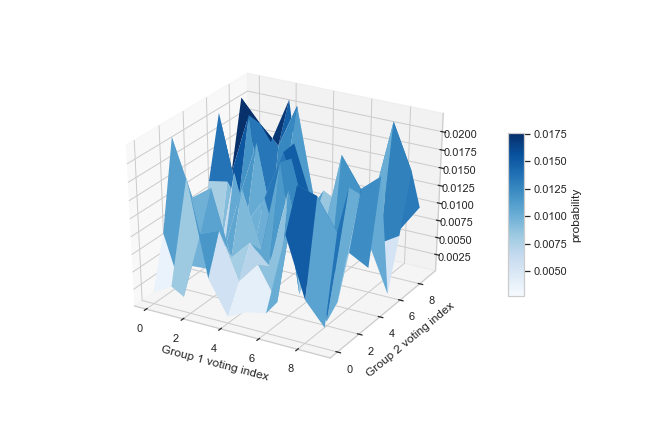
\includegraphics[width=\linewidth]{figures/2d_viz.png}
 \caption{Distribution of Probability over the 2D Hypercube for a Model in the $2 \times 2$ Case}
 \label{fig:2d_viz}
\end{figure}

Figure \ref{fig:3d_viz} shows the distribution of probability over the $2$D hypercube for a model in the $3 \times 2$ case. Since there are $3$ dimensions for demographic groups, Figure \ref{fig:3d_viz} presents the fourth dimension, probability, as directed arrows across a cross section of the dimensions. The colors of these arrows give the corresponding probability.

\begin{figure}[ht]\centering
 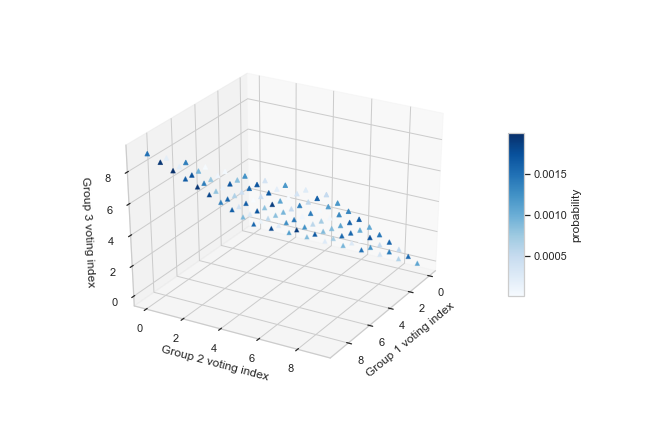
\includegraphics[width=\linewidth]{figures/3d_viz.png}
 \caption{Distribution of Probability over the 3D Hypercube for a Model in the $3 \times 2$ Case}
 \label{fig:3d_viz}
\end{figure}
